\documentclass[11pt]{article}
\usepackage{geometry}                % See geometry.pdf to learn the layout options. There are lots.
\geometry{letterpaper}                   % ... or a4paper or a5paper or ... 
%\geometry{landscape}                % Activate for for rotated page geometry
%\usepackage[parfill]{parskip}    % Activate to begin paragraphs with an empty line rather than an indent
\usepackage{graphicx}
\usepackage{amssymb}
\usepackage[danish]{babel}
\usepackage[utf8]{inputenc}
\usepackage{epstopdf}
\usepackage{hyperref}
\usepackage{parskip}
\hypersetup{
colorlinks = true,
linkcolor=black}


\DeclareGraphicsRule{.tif}{png}{.png}{`convert #1 `dirname #1`/`basename #1 .tif`.png}

\title{Clangton og Cant Specifikation}
\author{(Compiled Langton / Compiling Ant) \\ Pelle Juul Christensen}
%\date{}                                           % Activate to display a given date or no date

\begin{document}
\maketitle

\tableofcontents

\section{Clangton}
\subsection{Beskrivelse}

Clangton (compiled langton) er et programmeringsprog baseret på Langtons Myre, som i følge Gajardo et al. i stand til at simulere ethvert boolsk kredsløb.

Centralt i en Clangton program er start- og slutpositionen, samt bevægelsesfladen. ydermere tillader ind- og ud interaktion med brugeren og udvider dermed horisonten for mulige applikationer. For at lave mere avancerede programmer, eller blot for at gøre udvikling nemmere, er der implementeret del- og teleceller, hvilke er beskrevet senere i dette dokument. 

Ud over klassiske logiske operationer, så som AND, OR og NOT kan man med Clangton definere arbitrære operationer med udgangspunkt i reglerne for Langtons myre.

\subsection{Generelt}
Alle clangton kildekodefiler indeholder følgende blokke:
\begin{enumerate}
	\item størrelse
	\item startposition
	\item slutpostion
	\item bevægelsesfladen
	\item fra delceller
	\item til delceller
	\item fra teleceller
	\item til teleceller
	\item indcelle
	\item udcelle
\end{enumerate}

Blokke er separeret med / (skråstreg) og skal optræde i den definerede rækkefølge. For at mindske antallet af variable i den oversatte kode er alle positioner noteret med ét tal, som svarer til én celle. Celler er nummereret på følgende måde:

\begin{figure}[h]
\centering
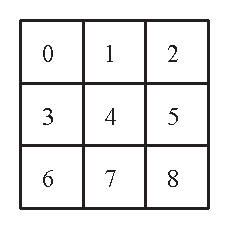
\includegraphics[scale=1]{plane}%
\end{figure}

En vigtig del af udvikling i Clangton er operationsrækkefølgen, hvilken foholder sig som følgende:

\begin{enumerate}
	\item standard bevægelse
	\item input
	\item ændring af retning og celletilstand
	\item delcelle
	\item teleceller
	\item output
\end{enumerate}

Desuden bør man notere sig at myren altid starter i opadgående retning.

\subsection{Definitioner}
\subsubsection{størrelse på bevægelsesflade}
Modtager et tal som svarer til bredden på bevægelsesfladen. Dette er brugt internet i den oversatte kode til at styre myrens position.

\subsubsection{start- og slutposition}
Disse felter siger mere eller mindre sig selv. En detalje er at myren ikke interagerer med startfeltet ved programstart, men dog interagerer myren med slutfeltet.

\subsubsection{bevægelsesfladen}
Bevægelsesfladen som myren traverserer, hvilket centralt definerer programmet. Her er cellers starttilstandr markeret med 1 eller 0, hvor 0 representerer et højresving og 1 et venstresving, begge relativt til myrens retning.

\subsubsection{til- og fra delceller}
Hvis myren bevæger sig ind i en fra-delcelle, vil denne skifte tilstand som normalt, herefter vil den tilsvarende til-delcelle skifte til samme tilstand som fra-delcellen.

\subsubsection{til- og fra teleceller}
Hvis myren bevæger sig ind i en til-telecelle, vil denne skifte tilstand som normalt, herefter vil myren blive transporteret til den tilsvarende til-celle, som ikke vil skifte tilstand.

\subsubsection{indceller}
Hvis myren bevæger sig ind i en incelle vil den stoppe og vente på input fra brugeren, og derefter forsætte afhængende af brugerens input.

\subsubsection{udceller}
Hvis myren bevæger sig ind i en udcelle vil cellen, vil denne skifte tilstand som normalt, efter tilstandsskiftet vil cellens tilstand blive udskrevet til brugeren.

\subsection{Eksempel}

\begin{verbatim}
# størrelse på bevægelsesfladen
3/
# startposition
4/
# slutposition
7/
# bevægelsesfladen
0,0,0, 0,0,0 ,0,0,0/
# fra-delceller
1/
# til-delceller
7/
# fra-teleceller
2,0/
# til-teleceller
7,7/
# indceller
1/
# udceller
7
\end{verbatim}

I dette eksempel har bevægelsesfladen en bredde på 3. Myren start på position 4 og slutter på position 7. Bevægelsesfladen er som udgangspunkt 'blank'. Celle 1 og 7 er et delcellepar, så når celle 1 skifter tilstand, følger celle 7 med. Der er to telecellepar $(2, 7)$ og $(0, 7)$, så ved ingang i celle 2 vil myren blive transporteret til celle 7, og ligeledes for celle 0. Celle 1 er bruger input hvor programmet bliver pauset og cellen tilstand bliver sat. Ved ingang i celle 7 bliver dennes tilstand printet, hvorefter programmet terminerer. 

Man kan tegne et afviklingsgraf for dette program hvor knuder viser myrens position og kanter er noteret med den forhenværende knudes tilstand:

\begin{figure}[h]
\centering
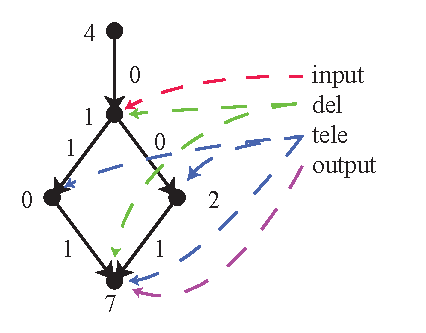
\includegraphics[scale=1]{graph}%
\end{figure}

\section{Cant}
Med en gyldig Clangton kildekode kan man vha. oversætteren cant (compiling ant) lave en eksekverbar fil. Syntaksen er som følgende:

\begin{verbatim}
./cant intput.cla output.c
\end{verbatim}

Det er vigtigt at man under brug af cant har 'main' filen liggende i samme mappe, som Cant. 

Cant oversætter Clangtonkodefilen til en C-kodefil, denne kan herefter oversættes med din yndlingsoversætter:

\begin{verbatim}
	gcc output.c -o mitProgram
\end{verbatim}

\section{ClangtonEdit}
ClangtonEdit er en simpel editor til clangton, hvis formål er at hjælpe med visualisering og udvikling af "større" Clangton programmer.

Ligesom Clangton-sproget er den centrale del af ClangtonEdit bevægelsesfladen. Ved at venstreklikke på en celle, bliver denne valgt og kan redigeres vha. toggle- og tekstboksene i højre side. Ved at højreklikke på en celle skifter dennes tilstand fra højre til venstre og vice versa.

Øverst i højre side kan ses hvilken celle der pt. er valgt. Straks nedenunder bevægelsesfladen kan man se hvilken celle musen i øjeblikket svæver over. Disse tal er en vigtig del af Clangtonudvikling siden de bruges som reference når man skal bruge del- og teleceller.

I midten til højre kan man specificere start og slut kordinat. \textbf{Det er vigtigt at man trykker 'retur' efter enhver redigering i en tekstboks, ellers vil ændringen ikke blive gemt}, dette gælder også for del- og tellecelletekstboksene.

Til slut kan man gemme sit program ved at trykke 'Save File' nederst til højre og derefter finde en fil at gemme til. For at simplificere oversættelse af sit program, anbefaler jeg at gemme det i samme mappe som 'cant' og 'main'. Standardenfilendelsen for Clangtonprogrammer er '.cla', men det er egentlig ligegyldigt, oversætteren er ligeglad.

\begin{figure}[h]
\centering
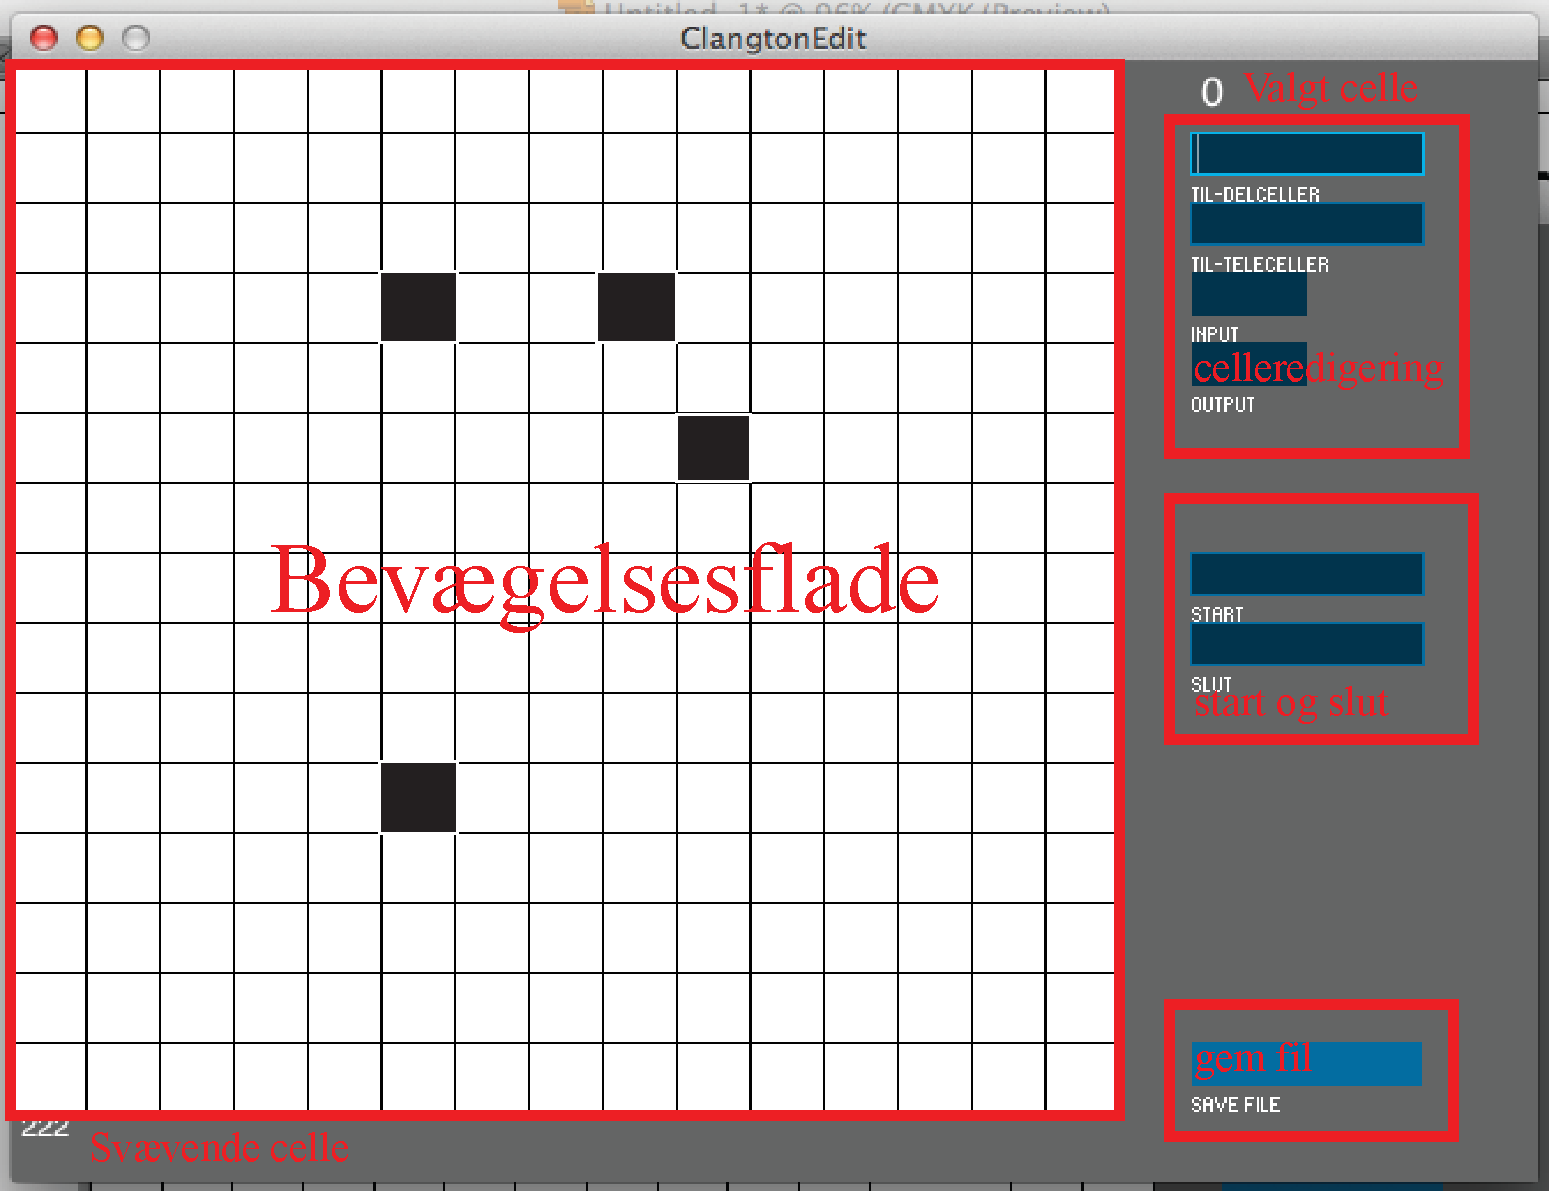
\includegraphics[scale=0.6]{clangtonedit}%
\end{figure}



\section{Links}
\href{http://en.wikipedia.org/wiki/Langton's_ant}{Wikipedia artikel om Langtons myre}

\href{http://www.dim.uchile.cl/~anmoreir/oficial/langton_dam.pdf}{Artikel om Langtons myres kompleksitet og universalitet}




\end{document}  